\begin{frame}
    \frametitle{D,F,G}

    \begin{itemize}
        \item 計算殘差
        \item 繪製殘差直方圖
        \item 針對$\ln(TOTEXP)$繪製
        \item 進行 Jarque-Bera 檢定
    \end{itemize}
\end{frame}

\begin{frame}[fragile]
    \frametitle{G,H 為例}
    從 $FOOD = PFOOD \times TOTEXP$得到 $FOOD$並估計
    \begin{lstlisting}
gen food = totexp*pfood
eststo est_g: reg food ln_totexp\end{lstlisting}

    \vfill
    建立計算彈性的函式(選擇性,也可以慢慢打)
    \begin{lstlisting}
capture program drop elas_g
program elas_g
    args total_ex est_name
    qui estimates restore `est_name'
    nlcom Elasticity: _b[ln_totexp] ///
        / (_b[_cons] + _b[ln_totexp]*log(`total_ex') )///
        , noheader
end
        
elas_g total_ex_p50 est_g
elas_g total_ex_p75 est_g\end{lstlisting}
\end{frame}

\begin{frame}[fragile]
    \frametitle{慢慢打版本}
    \begin{lstlisting}

qui estimates restore est_g
nlcom Elasticity: _b[ln_totexp] ///
    / (_b[_cons] + _b[ln_totexp]*log(total_ex_p50) )///
    , noheader     
nlcom Elasticity: _b[ln_totexp] ///
    / (_b[_cons] + _b[ln_totexp]*log(total_ex_p75) )///
    , noheader \end{lstlisting}

上面的 \texttt{total\_ex\_p50} 是先透過 \texttt{sum totexp, detail} ,再從中取得50, 70 百分位數\texttt{scalar total\_ex\_p75=r(p75)}
\end{frame}

\begin{frame}[fragile]
    \frametitle{G,H 為例 (續)}
    建立殘差
    \begin{lstlisting}
estimates restore est_g
predict res_h, residual\end{lstlisting}
    繪製殘差直方圖
    \begin{lstlisting}
histogram res_h, name("Q4_11_hist_3", replace)
graph export "Q4_11_hist_3.eps", name(Q4_11_hist_3) replace

twoway (scatter res_h ln_totexp ), name("Q4_11_scatter_3", replace)
graph export "Q4_11_scatter_3.eps", name("Q4_11_scatter_3") replace\end{lstlisting}
\end{frame}

\begin{frame}[allowframebreaks]
    \frametitle{H做圖結果}
    \begin{figure}
        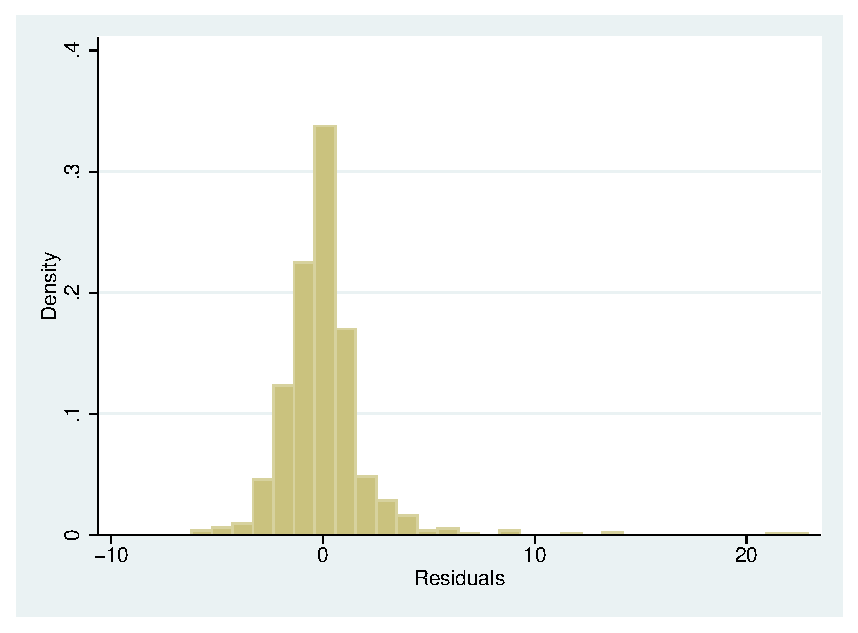
\includegraphics[width = 0.8\textwidth]{../Results/Q4_11_hist_3.eps}
    \end{figure}
    \begin{figure}
        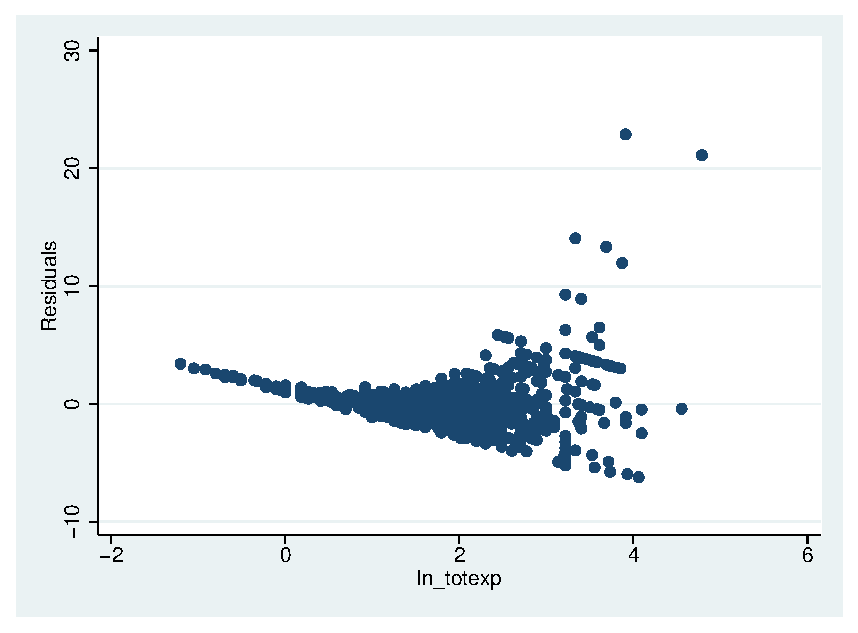
\includegraphics[width = 0.8\textwidth]{../Results/Q4_11_scatter_3.eps}
    \end{figure}
\end{frame}
